\section{Tour of the Systems}
There are different machines placed around the room, this section aims to give a brief overview of where each machine is located.

Captury Machine: This machine is located in the server rack on the right side of the observation room. The monitor, keyboard and mouse are located on the right side of the table facing the experiment room. The power button is located on the front of the machine behind a small swing window. The login information is provided on the inside of the swing window.

Windows Machines: The Dell tower PCs are number 1-3 going left to right of the room. PC1 is located facing the window to the outside, PC2 is the left most machine on the table facing the experiment room and PC3 is the middle machine on the table facing the experiment room.

There are different headsets available to the user however, the Meta Quest Pro is the recommended headset for the system. These headsets are usually located on top of the respective PCs, or located in the lockers on the back wall.

\section{Map of the System}
These diagrams show the layout of the system and how the data flows between the different machines.
\begin{figure}[H]
    \centering
    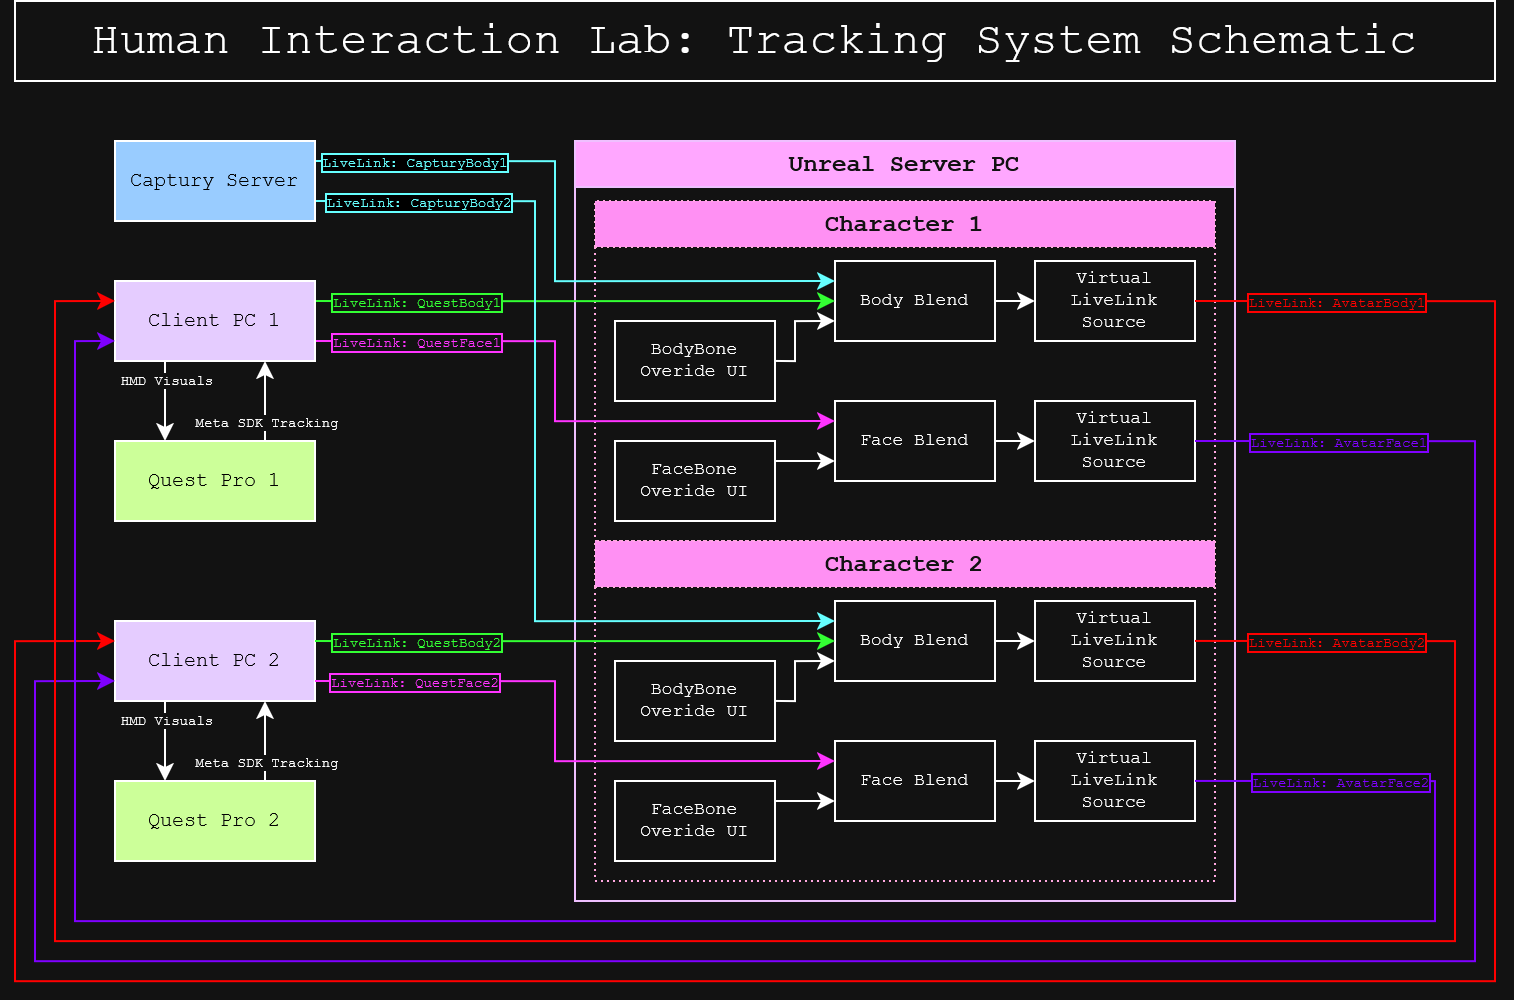
\includegraphics[width=\textwidth]{images/HILCircuitDiagram.png}
    \caption{Map of the System}
    \label{fig:system_map}
\end{figure}

\begin{figure}[H]
    \centering
    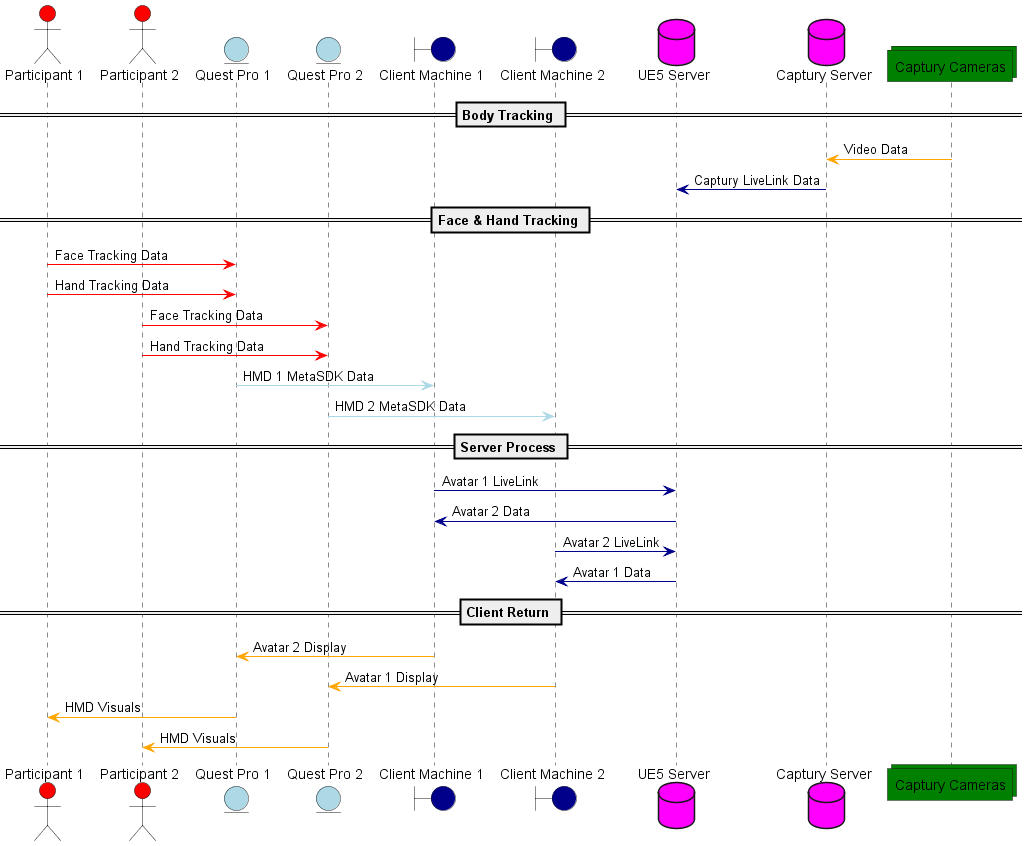
\includegraphics[width=\textwidth]{DataflowDiagram.png}
    \caption{A diagram to show the data flow of the system}
    \label{fig:system_map_alt}
\end{figure}
